\documentclass[a4paper,french]{paper}
\usepackage{../../../../../_assets/latex/5N_OPTO_ELEC}

%Informations about this document 
%------------------------------------------
\def\module{Opto-Electronique - S5}
\def\moduleAbrege{5N-027-SCI / OptoElec}
\def\annee{2024-2025}

\def\titre{Séance 5 / Photodétection}
\author{Julien VILLEMEJANE}

\subtitle{Séance 5}
\institution{LEnsE / Institut d'Optique Graduate School}

\title{\titre}
\begin{document} 
%Beginning First Page. 
%------------------------------------------
\enteteThematiqueObligatoire{}

\textit{Pour ce TD, on pourra s'appuyer sur la fiche résumée} : \href{https://lense.institutoptique.fr/ressources/Annee1/Electronique/fiches/2020_FR_Diodes_LED.pdf}{Diodes / LED / Photodiodes}

%Beginning Content. 
%------------------------------------------

%%%%%%%%%%%%%%%%%%%
%%%%%%%%%%%%%%%%%%%
\encadreTDExo{5.1 - Emettre une information lumineuse}{
En se basant sur une \textbf{LED IR} de type SFH415.

Proposer un montage émetteur permettant d'obtenir un flux lumineux sinusoïdal sans risque pour la LED, et donner les paramètres des différentes sources utilisées et des autres éléments du montage.
}

Il faut dans un premier temps s'intéresser aux données fournies par le constructeur pour savoir comment utiliser dans les meilleures conditions cette LED.

Il faut en particulier regarder les point suivants :

\begin{itemize}
	\item Courant maximal direct : 
	\item Tension inverse maximale ($V_R$) : $5\operatorname{V}$
	\item Tension directe ($V_F$) : $1.3\operatorname{V}$ @ $100\operatorname{mA}$
\end{itemize}

\qquad

On pourra utiliser le montage suivant pour piloter la LED : 

\begin{circuitikz}
	\draw (1,0) to [short, *-] (3,0)
		to[D=$LED$, -, invert] (3,2)
		to[R=$R_{LED}$, -] (3,4)
		to [short, -*, i<_=$I$] (0,4);
	\draw (3,0) to[short, -o] (4,0);
	
	% fleche
	\draw (0,0.5) edge[->] (0,3.5);
	\node (Ein) at (-1,2.25){$V_E$};

	\draw (0,0) to [short, *-] (1,0)
		node[ground](GND){};
	% fleche
	\draw (3.7,0.3) edge[->, green!40!black] (3.7,1.7); \node[text=green!40!black] (US) at (4,1){$V_F$};
\end{circuitikz}


%%%%%%%%%%%%%%%%%%%
%%%%%%%%%%%%%%%%%%%
\encadreTDExo{5.2 - Transmettre une information par la lumière}{
En se basant sur une \textbf{LED IR} de type SFH415 et une \textbf{photodiode} de type SFH229, on souhaite réaliser un système de transmission d'information par la lumière.

On se propose dans un premier temps d'utiliser le montage "simple" de photodétection.

\begin{center}
	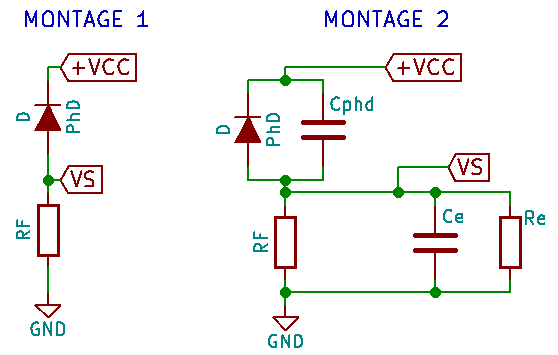
\includegraphics[width=7cm]{images/photodetection_simple_modele.png}
\end{center}

A quoi correspondent les deux montages proposés ?

Donner la fonction de transfert du montage en fonction du flux lumineux reçu.

Quelle est alors la limite en fréquence d'un tel montage ? Peut-on transmettre des données binaires ?
} 


On peut tout d'abord s'intéresser aux caractéristiques principales d'une photodiode :

\begin{itemize}
	\item tension inverse maximale / Reverse Voltage (p.2)
	\item puissance maximale admissible / Total Power Dissipation (p.2)
	\item courant photonique pour un éclairement particulier / Photocurrent (p.2)
	\item intervalle de longueurs d'ondes utilisable / Spectral range of sensibility (p.2)
	\item sensibilité spectrale / Spectral Sensibility (p.2)
	\item demi-angle / Half Angle (p.2)
	\item temps de réponse / Rise and Fall Time (p.3)
	\item tension direct / Forward Voltage (p.3)
	\item capacité parasite / Capacitance (p.3)
\end{itemize}

On peut également s'intéresser aux graphiques suivants : Relative Spectral Sensibility (p.4), Dark Current (p.4), Capacitance (p.5) et Directionnal Characteristics (p.5)

\qquad

\textbf{Montage 1}

Ce montage correspond au schéma de câblage d'une photodiode. La photodiode va imposer un courant proportionnel au flux lumineux reçu dans ce montage ($\Phi_e$). La résistance $R_F$ va alors servir à convertir ce courant (relativement faible) en une tension visualisable sur un oscilloscope par exemple.

Par application de la loi d'Ohms, le courant qui sort de la photodiode passe par la résistance $R_F$. On a donc : $V_S(t) = R_F \cdot I_{phd}(t)$.

De plus, $I_{phd}(t) = k \cdot \Phi_e(t)$, on a donc : $$\boxed{V_S(t) = k \cdot R_F \cdot \Phi_e(t)}$$

\qquad

\textbf{Montage 2}

Ce second montage correspond à la modélisation plus complète des éléments du montage 1.

On s'aperçoit expérimentalement que le système précédent n'a pas une amplitude constante quelque que soit la fréquence du signal lumineux émis.

Le phénomène observé peut s'expliquer par le fait que les éléments de mesure par exemple peuvent être modélisés par une impédance d'entrée ($R_e$) en parallèle avec une capacité ($C_e$).
D'une manière équivalente, on peut modéliser une photodiode (polarisée pour fonctionner en photodétecteur) comme une source de courant en parallèle avec une capacité ($C_{PHD}$).

\textbf{Etude du montage 2}

On supposera dans la suite de ce problème que le système est linéaire et que le flux lumineux reçu est une combinaison d'un flux constant et d'une somme de flux sinusoïdaux, pouvant s'écrire :

$$\phi_{lum}(t) = \Phi_{ambiant} + \sum_{i = 1}^{N} \phi_i \cdot sin(\omega_i \cdot t)$$

On peut décomposer le signal $\phi_{lum}(t)$ en $N+1$ sources indépendantes : $\Phi_{ambiant}$ source continue et $N$ sources de fréquence $f_i$. 
		
		Comme le système est linéaire, on peut alors appliquer le théorème de superposition. On peut alors sommer les causes de chacune des sources indépendantes.
		
		On peut alors réaliser l'étude en polarisation indépendamment de l'étude en petits signaux, en s'intéressant aux 2 montages suivants :

\begin{center}
	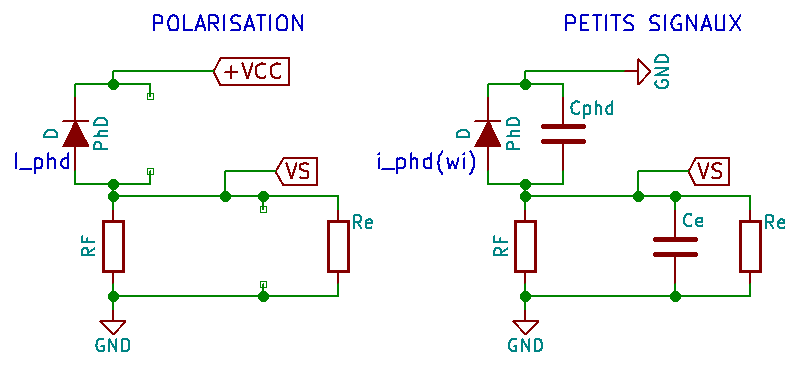
\includegraphics{images/photodetection_simple_modele_corr.png}
\end{center}

\textbf{\textit{Cas continu}}

Dans le cas de l'étude en continu (polarisation), on obtient : 
$V_{Scont} = (R_F // R_e) \cdot I_{phd} = (R_F // R_e) \cdot k \cdot \Phi_{ambiant}$


\textbf{\textit{Cas "petits signaux"}}

L'ensemble des éléments sont en parallèle. On obtient donc la relation suivante : $V_S(f_i) = k \cdot \phi_i \cdot (R_e // R_F // C_{phd} // C_e)$.
	
	En appelant $Y = 1/(R_e // R_F // C_{phd} // C_e)$, on obtient $V_S(f_i) = k \cdot \phi_i / Y$ avec :
	
	$$Y = \frac{1}{R_F} + \frac{1}{R_e} + j \cdot (C_{phd} + C_e) \cdot \omega_i$$
	
	$$Y = \frac{R_e + R_F}{R_F \cdot R_e} \cdot (1 + j \cdot \omega_i \cdot (C_{phd} + C_e) \cdot \frac{R_F \cdot R_e}{R_e + R_F})$$
	
	On obtient alors :
	
	$$\boxed{\frac{V_S(f_i)}{\phi_i} = k \cdot \frac{R_F \cdot R_e}{R_e + R_F} \cdot \frac{1}{(1 + j \cdot \omega_i \cdot (C_{phd} + C_e) \cdot \frac{R_F \cdot R_e}{R_e + R_F})}}$$
	
	On retrouve alors le comportement d'un filtre passe-bas dont la fréquence de coupure est $$\boxed{\omega_0 = \frac{R_e + R_F}{R_F \cdot R_e \cdot (C_{phd} + C_e)}}$$.


%%%%%%%%%%%%%%%%%%%
%%%%%%%%%%%%%%%%%%%
\encadreTDExo{5.3 - Transmettre une information par la lumière - transimpédance}{
En se basant sur une \textbf{LED IR} de type SFH415 et une \textbf{photodiode} de type SFH229, on souhaite réaliser un système de transmission d'information par la lumière.

On se propose dans un premier temps d'utiliser le montage de photodétection de type transimpédance.

\begin{center}
	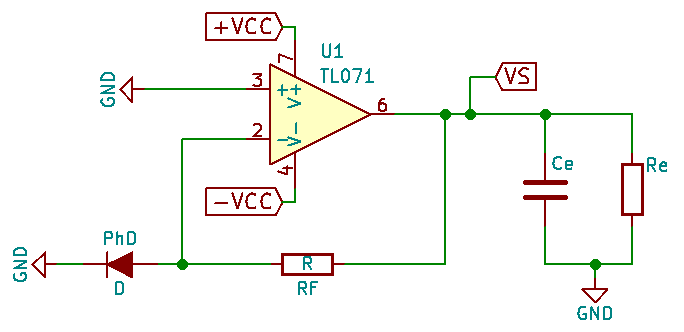
\includegraphics[width=8cm]{images/photodetection_transimpedance.png}
\end{center}

Donner la fonction de transfert du montage en fonction du flux lumineux reçu.

Quelle est alors la limite en fréquence d'un tel montage ? Peut-on transmettre des données binaires ?
}

On se basant sur les hypothèses habituelles pour un amplificateur intégré, on se trouve dans le cas d'un fonctionnement linéaire ($V^+ = V^-$) et on pourra supposer les courants d'entrée négligeables. On obtient alors que : $$\boxed{V_S = -R_F \cdot I_{PHD}}$$

\qquad

Même en modélisant le système de mesure par une capacité $C_e$ et une résistance $R_e$ en parallèle, on s'aperçoit que ces éléments n'interviennent plus dans le calcul de la fonction de transfert. Le courant fourni à ces éléments ne provient pas de la photodiode (contrairement au montage 1) mais provient de l'ALI (et de son alimentation).

\qquad

Expérimentalement, cependant, on retrouve un phénomène passe-bas, inexpliqué par les relations obtenues précédemment (voir thème 2 de TP).


%%%%%%%%%%%%%%%%%%%
%%%%%%%%%%%%%%%%%%%
\encadreTDExo{5.B1 - Modéliser le montage transimpédance}{
Dans l'exemple précédent, nous avons supposé l'amplificateur linéaire idéal. 

On prendra le modèle suivant pour l'amplificateur linéaire :

$$V_S = \frac{A_0}{1 + j \cdot \frac{\omega}{\omega_0}} \cdot (V^+ - V^-)$$

Calculer la fonction de transfert $T(j\cdot \omega) = V_S /  i_{PHD}$ du montage suivant :
} 


\begin{figure}[!h]
\centering
\begin{circuitikz} 
	\node [op amp](A1) at (0,0){\texttt{ALI1}};
	\draw (A1.-) to[short] ++(-.5,0) coordinate(A) to[short] ++(0,1.5) coordinate(B) to[R=$R_F$, i=$i_R$] (B -| A1.out) to[short, -*] (A1.out);
	\draw (A1.- -| -5,0) node[ground]{};
	\draw (A1.- -| -5,0) to[I, invert, i=$i_{Phd}$, *-*] (A);
	\draw (A1.- -| -5,0) -- ++(0,1.5) to[C, l=$C_{Phd}$, i=$i_C$, -*] (B);
	\draw (A1.+) to[short] ++(0,-0.5) node[ground]{};
	\draw (A1.out) -- ++(1,0) coordinate(D);
	\draw (2.2,-2.1) edge[->, color={red}] (2.2,-0.3);
	\node[text={red}] (Vs) at (1.7,-1.2){$V_s$}; 
	\draw (D) -- ++(1,0) to[C,l=$C_{e}$, *-*] ++(0,-2.5) coordinate(G);
	\draw (G) node[ground]{};
	\draw (G) -- ++(2,0) to[R,l=$R_e$] ++(0,2.5) -- ++(-2,0);
\end{circuitikz}
\end{figure}

Si on s'intéresse à présent au modèle un peu plus réaliste d'un ALI, on peut alors calculer la fonction de transfert du montage précédent de manière à interpréter les résultats expérimentaux obtenus.

On a $V^+ = 0$.

\textbf{Calcul de $V^-$}

Loi des noeuds : $i_{PHD} + i_C = i_R$  (on supposera $i^- = 0$).

\textit{\textbf{Calcul de $i_R$}}

Loi des mailles : $V^- - R_F \cdot i_R - V_S = 0$

Ainsi : $\boxed{i_R = \frac{V^- - V_S}{R_F}}$

\textit{\textbf{Calcul de $i_C$}}

On posera $Z_C = \frac{1}{C_{PHD} \cdot \omega}$

Loi des mailles :  $V^- + Z_C \cdot i_C = 0$

Ainsi : $\boxed{i_C = \frac{-V^-}{Z_C}}$

\textit{\textbf{Calcul de $V^-$}}

$i_{PHD} + \frac{-V^-}{Z_C} = \frac{V^- - V_S}{R_F}$

Ainsi : $i_{PHD} = V^- \cdot (1/R_F + 1/Z_C) - V_S/R_F$

On obtient alors : $$\boxed{V^- = \frac{1}{1 + j \cdot R_F \cdot C_{PHD} \cdot \omega} \cdot (R_F \cdot i_{PHD} + VS)}$$

\textbf{Calcul de $V_S$}

On a $V_S = A(j\omega) \cdot (V^+ - V^-)$.

On obtient alors : $$V_S = - A(j\omega) \cdot \frac{V_S + R_F \cdot i_{PHD}}{1 + j R_F C_{PHD} \omega}$$

On obtient ainsi la fonction de transfert suivante : 
$$\boxed{\frac{V_S}{i_{PHD}} = \frac{- A(j\omega) \cdot R_F}{1 + A(j\omega) + j R_F C_{PHD} \omega}}$$

\textbf{Calcul complet}

En remplaçant $A(j\omega)$ par $\frac{A_0}{1 + j \cdot \frac{\omega}{\omega_0}}$, on obtient alors la fonction de transfert suivante :

$$boxed{\frac{V_S}{i_{PHD}} = \frac{- A_0 \cdot R_F}{(1 + j R_F C_{PHD} \omega) \cdot (1 + j \omega/\omega_0) + A_0}}$$

Ce système correspond alors à un filtre passe-bas du second ordre. Selon les valeurs de $R_F$, $C_{PHD}$, $A_0$ et $\omega_0$, il peut y avoir une résonance (voir Thème 2 de TP).


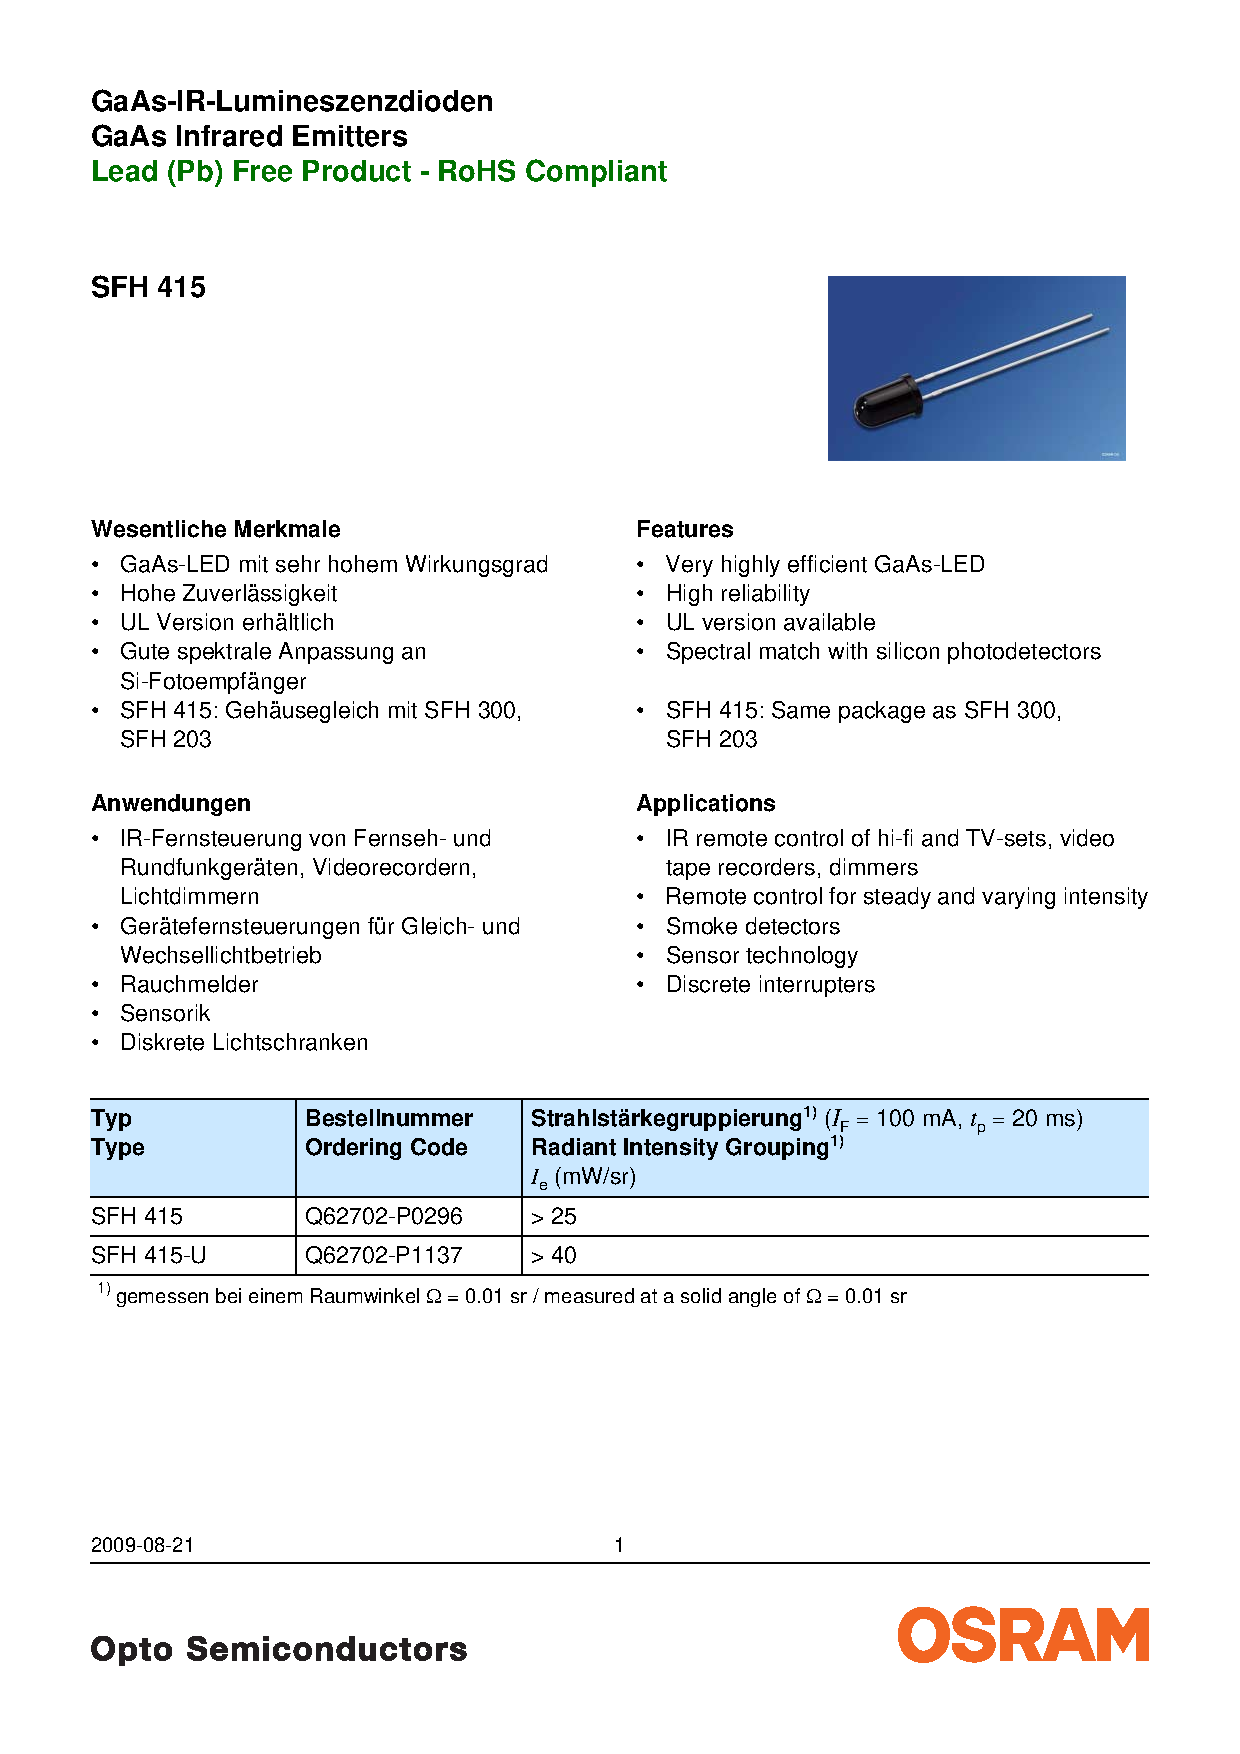
\includepdf[pages=1-3]{docs/SFH415.pdf}
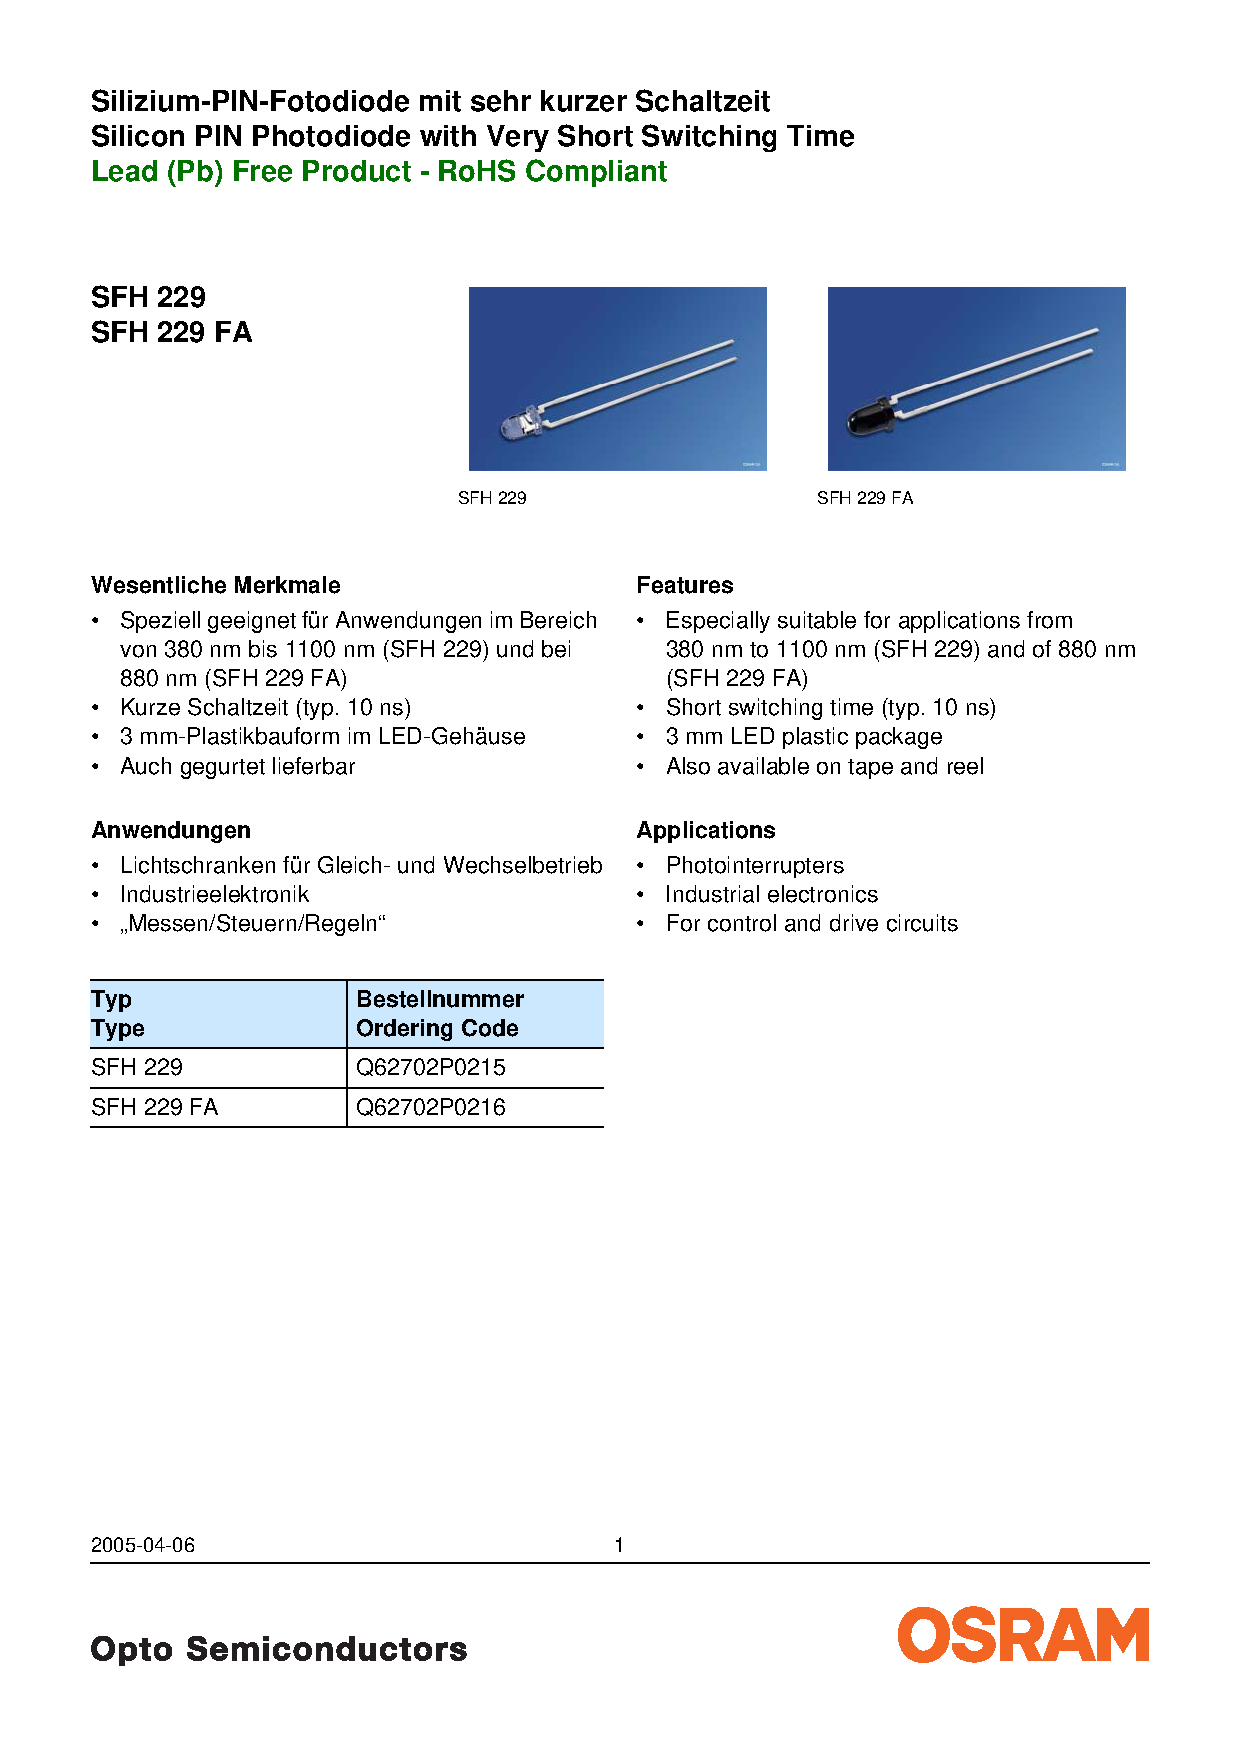
\includepdf[pages=1-5]{docs/SFH229.pdf}

\end {document}